%********************************************************************
% Appendix
%*******************************************************
% If problems with the headers: get headings in appendix etc. right
%\markboth{\spacedlowsmallcaps{Appendix}}{\spacedlowsmallcaps{Appendix}}
\chapter{Appendix B: Supplementary Information of Chapter 4}

\begin{refsection}[referencesCh3]
\section{Cattle organic waste composition} \label{ApBcomp_dist}
To calculate the distribution functions of the different compounds of the cattle organic waste, 37 data sets for cattle organic waste compositions from 20 bibliographic references were evaluated. Table \ref{table:dig_compt_stats} collects the main statistical parameters of the data, and Table \ref{table:refs} shown the data obtained from literature.

\section{Distribution functions of elements from cattle waste}

The kernel density estimation (KDE) method is used to fit the probability function to data distribution and to determine the probability density distributions of calcium, nitrogen, phosphorus, potassium, ammonia/total nitrogen, and phosphate/total phosphorus. As histograms, KDE is a non-parametric way to estimate the probability density function of a random variable. However, in the KDE method, kernels are functions associated with each data set. Thus, the unknown density function can be computed as the weighted sum of these functions \citep{Duong}. 

The calculation procedure is divided into three steps. First, cattle organic waste composition data are collected from the literature. Second, the KDEs of all compounds are estimated, and finally, distribution functions are fitted, using the kernel density estimations to validate the chosen distribution. The probability density distributions which best fit the data distribution are normal distribution functions for the distribution of nitrogen as in Figure \ref{fig:N_KDE}, ammonia/total nitrogen molar ratio as observed in Figure \ref{fig:NH4_frac_KDE}, and phosphorus as shown in Figure \ref{fig:P_KDE}. Lognormal distribution functions are the best fit for phosphate/total phosphorus molar ratio as in Figure \ref{fig:PO4_frac_KDE}, calcium, as shown in Figure \ref{fig:Ca_KDE}, and potassium as observed in Figure \ref{fig:K_KDE}.

\begin{sidewaystable}
	\centering
	\caption{Statistical summary of cattle organic waste composition. Data from \protect\citep{Alburquerque,Bolzonella,Seppala,Gell,Normak,Sorensen,Tampere,Moset,Zheng,Xia,Moller,WRAP,ADAS,Risgberg,Ledda,Kirchmann,Moller2,Walsh,Loes,Martin2}.} \label{table:dig_compt_stats}
	\resizebox{0.9\columnwidth}{!}{
	\begin{tabular}{ c c c c c c c c c c c}
		\toprule
		&DM		&C		&Ca		&K		&N		&P		&\multirow{2}{*}{\Large{$\frac{\text{Ca}^{\text{2+}}}{\text{Total Ca}}$}}	&\multirow{2}{*}{\Large{$\frac{\text{K}^{\text{+}}}{\text{Total K}}$}}	&\multirow{2}{*}{\Large{$\frac{\text{N-NH}^{+}_{4}}{\text{Total N}}$}}	&\multirow{2}{*}{\Large{$\frac{\text{P-PO}^{3-}_{4}}{\text{Total P}}$}}	\\	
		&(\% mass)		&(\% mass)		&(\% mass)		&(\% mass)		&(\% mass)		&(\% mass)		&	&	&	&	\\ \midrule
		count		&36		&6		&9		&12		&35		&24		&1			&1		&31			&13			\\ 
		mean		&5.858	&2.478	&0.117	&0.253	&0.384	&0.059	&0.154		&1.000	&0.590		&0.541		\\ 
		std		&1.778	&0.946	&0.027	&0.158	&0.133	&0.038	&NaN		&NaN	&0.117		&0.159		\\ 
		min		&2.624	&1.200	&0.080	&0.084	&0.114	&0.005	&0.154		&1.000	&0.348		&0.216		\\ 
		25.00\%	&4.610	&1.719	&0.100	&0.148	&0.299	&0.032	&0.154		&1.000	&0.516		&0.421		\\ 
		50.00\%	&5.668	&2.788	&0.110	&0.223	&0.399	&0.048	&0.154		&1.000	&0.616		&0.597		\\ 
		75.00\%	&7.362	&3.194	&0.129	&0.276	&0.449	&0.080	&0.154		&1.000	&0.666		&0.671		\\ 
		max		&9.200	&3.400	&0.165	&0.635	&0.789	&0.164	&0.154		&1.000	&0.820		&0.700		\\ \bottomrule
	\end{tabular}}
\end{sidewaystable}

%\begin{sidewaystable}
\begin{table}
	\centering
	\caption{Data obtained from literature.} \label{table:refs}
%	\resizebox{\columnwidth}{!}{
	\begin{adjustbox}{scale=0.65,center}
	\begin{tabular}{@{}ccccccccccc@{}}
		\toprule
		\begin{tabular}[c]{@{}c@{}}Dry matter\\ (\% wt)\end{tabular} & \begin{tabular}[c]{@{}c@{}}N\\ (\% wt)\end{tabular} & \begin{tabular}[c]{@{}c@{}}P\\ (\% wt)\end{tabular} & \begin{tabular}[c]{@{}c@{}}K\\ (\% wt)\end{tabular} & \begin{tabular}[c]{@{}c@{}}C\\ (\% wt)\end{tabular} & \begin{tabular}[c]{@{}c@{}}Ca\\ (\% wt)\end{tabular} & \begin{tabular}[c]{@{}c@{}}PO4\\ ratio\end{tabular} & \begin{tabular}[c]{@{}c@{}}NH4/N\\ ratio\end{tabular} & \begin{tabular}[c]{@{}c@{}}Ca2+/Ca\\ ratio\end{tabular} & \begin{tabular}[c]{@{}c@{}}K+/K\\ ratio\end{tabular} & Reference                                                                         \\ \midrule
		7.35                                                         & 0.52                                                & 0.15                                                & 0.64                                                & 2.98                                                & 0.17                                                 & 0.35                                                & 0.63                                                  &                                                         &                                                      & \cite{Moller}                                                             \\
		4.90                                                         & 0.79                                                & 0.04                                                & 0.16                                                &                                                     & 0.13                                                 & 0.33                                                & 0.68                                                  & 0.15                                                    & 1                                                    & \cite{WRAP}                                                                              \\
		7.40                                                         & 0.42                                                & 0.03                                                & 0.23                                                &                                                     &                                                      &                                                     & 0.38                                                  &                                                         &                                                      & \cite{ADAS}            \\
		6.50                                                         & 0.45                                                &                                                     &                                                     &                                                     &                                                      &                                                     & 0.60                                                  &                                                         &                                                      & \cite{ADAS}            \\
		5.58                                                         & 0.46                                                &                                                     &                                                     &                                                     &                                                      &                                                     & 0.64                                                  &                                                         &                                                      & \cite{ADAS}            \\
		4.49                                                         & 0.51                                                & 0.05                                                & 0.12                                                &                                                     &                                                      &                                                     & 0.82                                                  &                                                         &                                                      & \cite{ADAS}            \\
		8.47                                                         & 0.55                                                & 0.05                                                &                                                     &                                                     &                                                      & 0.67                                                & 0.56                                                  &                                                         &                                                      & \cite{ADAS}            \\
		5.69                                                         & 0.35                                                & 0.04                                                &                                                     &                                                     &                                                      & 0.70                                                & 0.65                                                  &                                                         &                                                      & \cite{ADAS}            \\
		8.30                                                         & 0.57                                                & 0.05                                                &                                                     &                                                     &                                                      & 0.64                                                & 0.50                                                  &                                                         &                                                      & \cite{ADAS}            \\
		6.75                                                         & 0.37                                                & 0.03                                                &                                                     &                                                     &                                                      & 0.57                                                & 0.64                                                  &                                                         &                                                      & \cite{ADAS}           \\
		3.80                                                         & 0.40                                                & 0.03                                                &                                                     &                                                     &                                                      & 0.70                                                & 0.67                                                  &                                                         &                                                      & \cite{ADAS}            \\
		5.50                                                         & 0.35                                                & 0.03                                                &                                                     &                                                     &                                                      & 0.60                                                & 0.45                                                  &                                                         &                                                      & \cite{ADAS}            \\
		7.99                                                         & 0.45                                                & 0.03                                                &                                                     &                                                     &                                                      & 0.62                                                & 0.55                                                  &                                                         &                                                      & \cite{ADAS}            \\
		7.52                                                         & 0.41                                                & 0.03                                                &                                                     &                                                     &                                                      & 0.54                                                & 0.58                                                  &                                                         &                                                      & \cite{ADAS}            \\
		7.40                                                         & 0.34                                                &                                                     &                                                     & 3.40                                                &                                                      &                                                     & 0.65                                                  &                                                         &                                                      & \cite{Risgberg}                               \\
		6.10                                                         & 0.41                                                &                                                     &                                                     & 2.60                                                &                                                      &                                                     & 0.68                                                  &                                                         &                                                      & \cite{Risgberg}                                \\
		4.80                                                         & 0.27                                                & 0.05                                                & 0.36                                                &                                                     &                                                      & 0.22                                                & 0.35                                                  &                                                         &                                                      & \cite{Seppala}                                  \\
		4.12                                                         & 0.20                                                &                                                     &                                                     &                                                     &                                                      &                                                     & 0.52                                                  &                                                         &                                                      & \cite{Alburquerque}                   \\
		7.84                                                         & 0.25                                                &                                                     &                                                     &                                                     &                                                      &                                                     & 0.38                                                  &                                                         &                                                      & \cite{Alburquerque}                             \\
		2.62                                                         & 0.15                                                &                                                     &                                                     &                                                     &                                                      &                                                     & 0.53                                                  &                                                         &                                                      & \cite{Alburquerque}                             \\
		7.00                                                         & 0.34                                                & 0.16                                                &                                                     &                                                     &                                                      & 0.42                                                & 0.52                                                  &                                                         &                                                      & \cite{Bolzonella}                            \\
		6.10                                                         & 0.20                                                &                                                     &                                                     &                                                     &                                                      &                                                     &                                                       &                                                         &                                                      & \cite{Gell}                                \\
		6.24                                                         & 0.47                                                &                                                     &                                                     &                                                     &                                                      &                                                     & 0.42                                                  &                                                         &                                                      & \cite{Moset}                                \\
		7.20                                                         & 0.36                                                & 0.08                                                &                                                     &                                                     &                                                      &                                                     & 0.51                                                  &                                                         &                                                      & \cite{Ledda}                                \\
		& 0.27                                                & 0.06                                                & 0.08                                                &                                                     & 0.13                                                 &                                                     &                                                       &                                                         &                                                      & \cite{Kirchmann} \\
		9.20                                                         & 0.40                                                & 0.06                                                & 0.43                                                & 3.27                                                &                                                      &                                                     &                                                       &                                                         &                                                      & \cite{Moller2}        \\
		5.20                                                         & 0.11                                                & 0.01                                                & 0.09                                                & 1.42                                                & 0.10                                                 &                                                     &                                                       &                                                         &                                                      & \cite{Walsh}         \\
		4.40                                                         &                                                     &                                                     &                                                     &                                                     &                                                      &                                                     &                                                       &                                                         &                                                      & \cite{Zheng}                                 \\
		4.65                                                         & 0.29                                                &                                                     &                                                     &                                                     &                                                      &                                                     & 0.62                                                  &                                                         &                                                      & \cite{Sorensen}                                           \\
		4.82                                                         & 0.31                                                &                                                     &                                                     &                                                     &                                                      &                                                     & 0.67                                                  &                                                         &                                                      & \cite{Sorensen}                                           \\
		3.50                                                         & 0.43                                                & 0.08                                                & 0.22                                                &                                                     & 0.11                                                 &                                                     & 0.72                                                  &                                                         &                                                      & \cite{Tampere}                                                        \\
		3.80                                                         & 0.44                                                & 0.08                                                & 0.22                                                &                                                     & 0.08                                                 &                                                     & 0.73                                                  &                                                         &                                                      & \cite{Tampere}                                                        \\
		3.20                                                         & 0.43                                                & 0.08                                                & 0.24                                                &                                                     & 0.10                                                 &                                                     & 0.77                                                  &                                                         &                                                      & \cite{Tampere}                                                       \\
		3.00                                                         & 0.24                                                & 0.03                                                &                                                     & 1.20                                                & 0.09                                                 &                                                     & 0.63                                                  &                                                         &                                                      & \cite{Loes}                                                                 \\
		9.11                                                         & 0.55                                                & 0.09                                                &                                                     &                                                     &                                                      & 0.67                                                & 0.56                                                  &                                                         &                                                      & \cite{Martin2}                                                                    \\
		4.70                                                         & 0.40                                                & 0.08                                                & 0.25                                                &                                                     & 0.15                                                 &                                                     & 0.72                                                  &                                                         &                                                      & \cite{Normak}                                                              \\
		5.65                                                         &                                                     &                                                     &                                                     &                                                     &                                                      &                                                     &                                                       &                                                         &                                                      & \cite{Xia}                                                                   \\ \bottomrule
	\end{tabular}
%	}
	\end{adjustbox}
\end{table}

\newpage

\begin{figure}[p]
	\centering	
	\begin{subfigure}[t]{0.45\textwidth}
		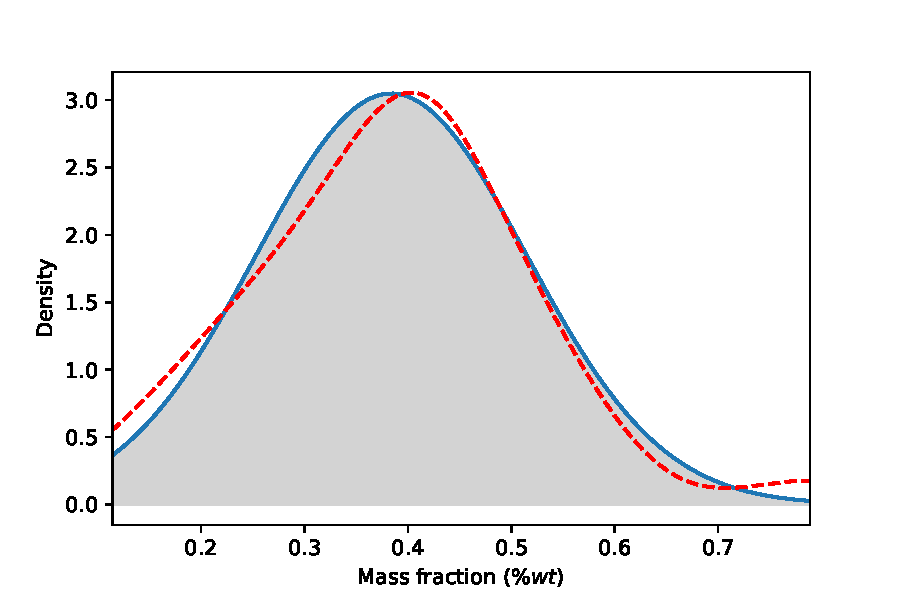
\includegraphics[width=\linewidth]{gfx/AppendixB/N_dist.pdf} 
		\caption{Nitrogen mass fraction (wet basis).}
		\label{fig:N_KDE}
	\end{subfigure}
	\qquad
	\begin{subfigure}[t]{0.45\textwidth}
		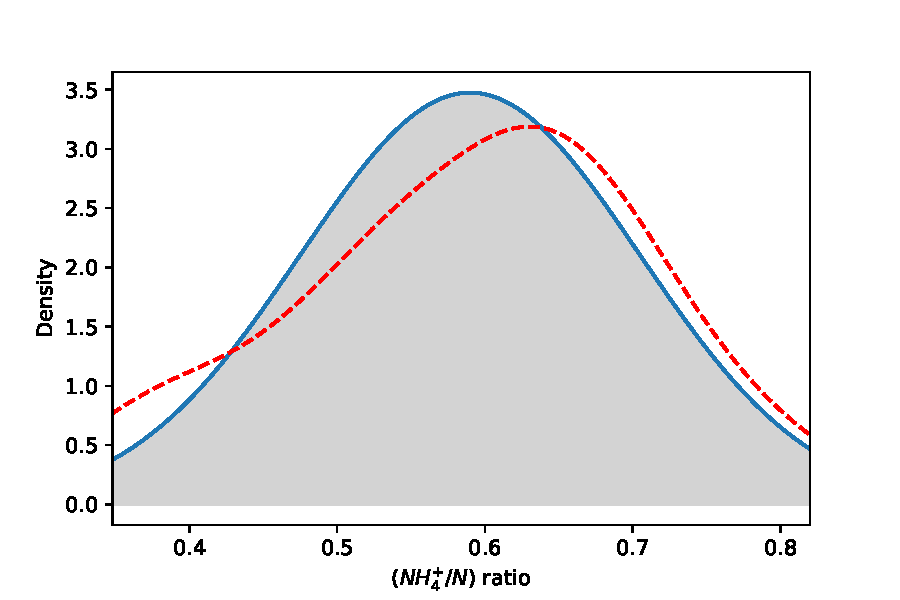
\includegraphics[width=\linewidth]{gfx/AppendixB/NH4_frac_dist.pdf}
		\caption{Ammonia/nitrogen ratio (mass basis).}
		\label{fig:NH4_frac_KDE}
	\end{subfigure}
	
	\begin{subfigure}[t]{0.45\textwidth}
		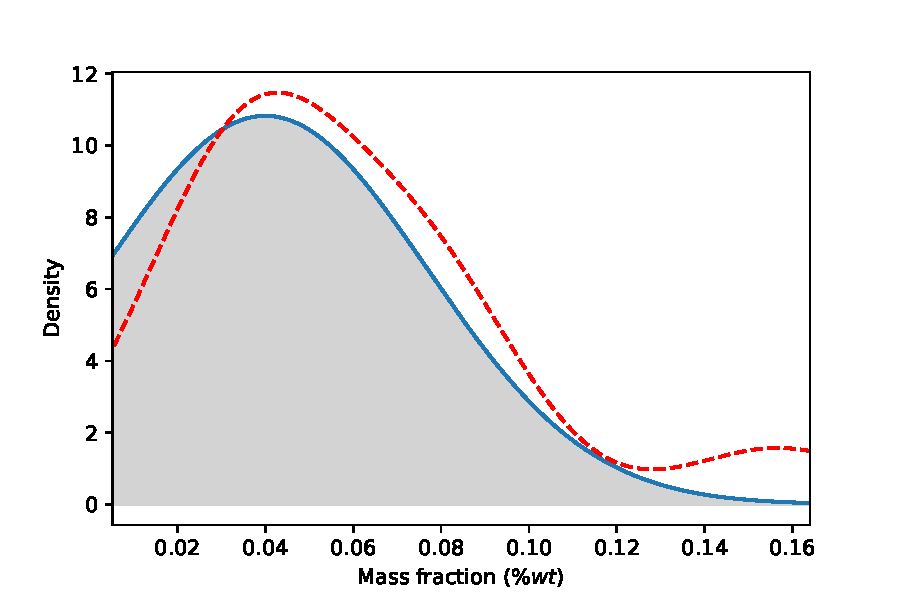
\includegraphics[width=\linewidth]{gfx/AppendixB/P_dist.pdf}
		\caption{Phosphorus mass fraction (wet basis).}
		\label{fig:P_KDE}
	\end{subfigure}
	\qquad
	\begin{subfigure}[t]{0.45\textwidth}
		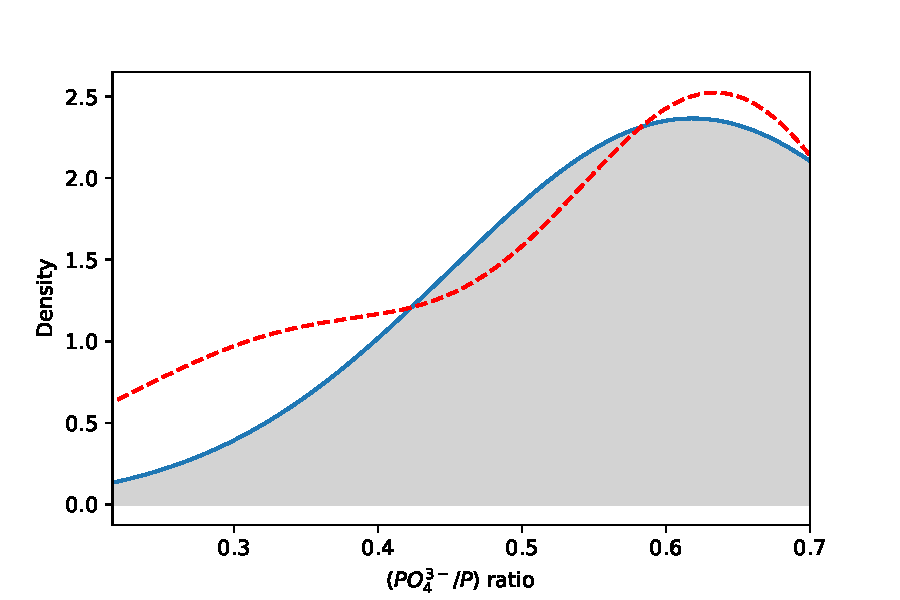
\includegraphics[width=\linewidth]{gfx/AppendixB/PO4_frac_dist.pdf}
		\caption{Phosphate/phosphorus ratio (mass basis).}
		\label{fig:PO4_frac_KDE}
	\end{subfigure}
	
	\begin{subfigure}[t]{0.45\textwidth}
		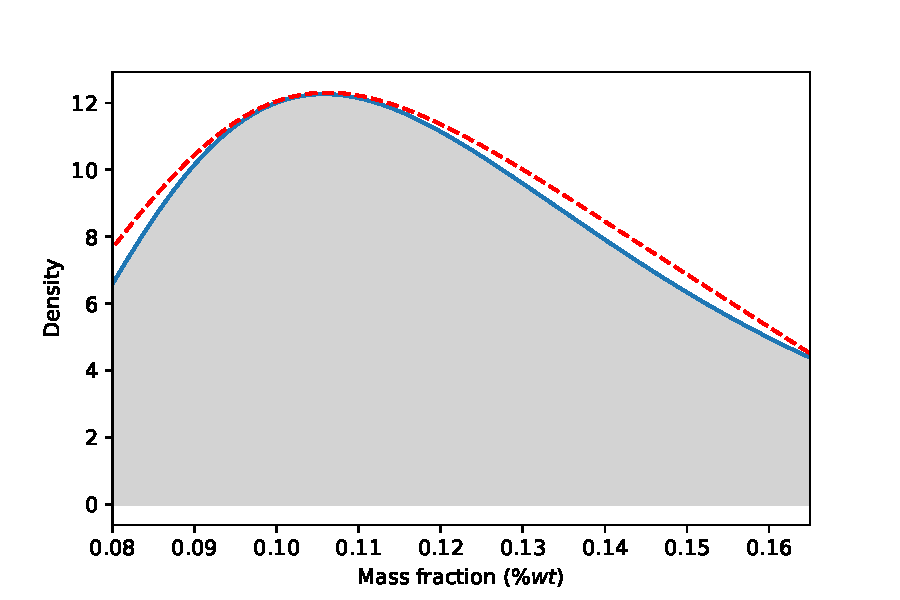
\includegraphics[width=\linewidth]{gfx/AppendixB/Ca_dist.pdf}
		\caption{Calcium mass fraction (wet basis).}
		\label{fig:Ca_KDE}
	\end{subfigure}
	\qquad
	\begin{subfigure}[t]{0.45\textwidth}
		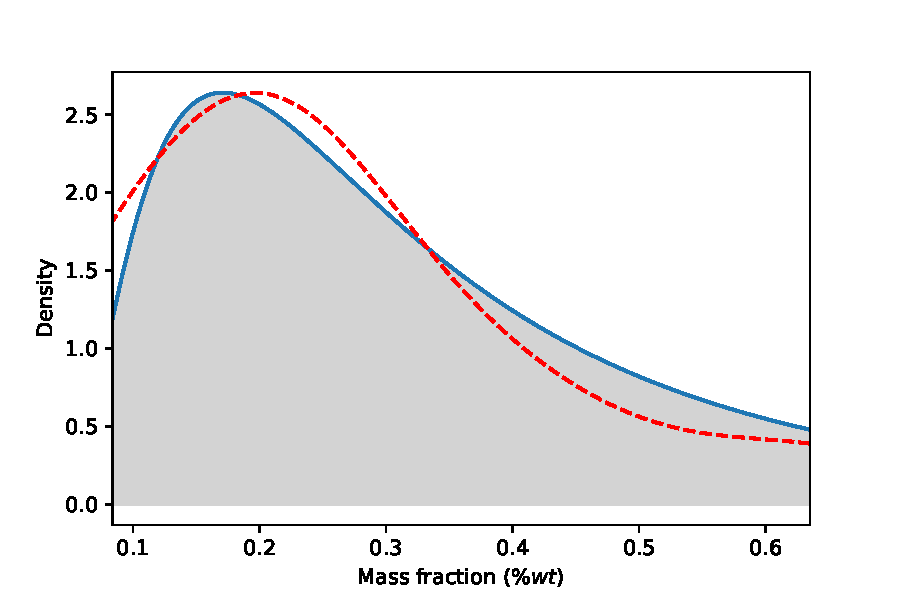
\includegraphics[width=\linewidth]{gfx/AppendixB/K_dist.pdf}
		\caption{Potassium mass fraction (wet basis).}
		\label{fig:K_KDE}
	\end{subfigure}
	\caption{Kernel density estimation (red dashed line) and probability density distribution (blue solid line) for the evaluated components in cattle organic waste.}
	\label{fig:components_distributions}
\end{figure}

%\section{Distribution functions of elements from cattle waste}
%
%The kernel density estimation (KDE) method is used to fit the probability function to data distribution and to determine the probability density distributions of calcium, nitrogen, phosphorus, potassium, ammonia/total nitrogen, and phosphate/total phosphorus. As histograms, KDE is a non-parametric way to estimate the probability density function of a random variable. However, in the KDE method, kernels are functions associated with each data set. Thus, the unknown density function can be computed as the weighted sum of these functions \citep{Duong}. 
%
%The calculation procedure is divided into three steps. First, cattle organic waste composition data are collected from the literature. Second, the KDEs of all compounds are estimated, and finally, distribution functions are fitted, using the kernel density estimations to validate the chosen distribution. The probability density distributions which best fit the data distribution are normal distribution functions for the distribution of nitrogen as in Figure \ref{fig:N_KDE}, ammonia/total nitrogen molar ratio as observed in Figure \ref{fig:NH4_frac_KDE}, and phosphorus as shown in Figure \ref{fig:P_KDE}. Lognormal distribution functions are the best fit for phosphate/total phosphorus molar ratio as in Figure \ref{fig:PO4_frac_KDE}, calcium, as shown in Figure \ref{fig:Ca_KDE}, and potassium as observed in Figure \ref{fig:K_KDE}.

\clearpage

\section{Thermodynamic modeling of the carbonates system} \label{Carbonates}
To calculate the total carbonate content, the concept of defining alkalinity will be used. The formal definition of total alkalinity is the capacity of a solution to buffer changes in pH that would make the solution more acidic.
From the perspective of charge balance, total alkalinity can be considered as a measure of the number of protons that can be accepted by the proton acceptors present in the dissolution. Therefore, total alkalinity, $TA$, is calculated as the excess of proton acceptors over donors with respect to a chosen zero level of protons, as in Eq. \ref{eq:gen_alk}:
\begin{align} 
& TA = \text{proton acceptors} - \text{proton donors} \label{eq:gen_alk}
\end{align}
Note that the distribution of different species for various systems, such as carbonic acid and phosphoric acid, depend on pH, and the contribution of each species to alkalinity, is a function of its electrical charge. For our case, the chemical systems considered are water, carbonic acid, phosphoric acid, and ammonia systems
%, as shown in Table \ref{table:pK}.

A zero level of protons is a reference system defined by choosing a certain chemical compound for each system at a certain pH selected arbitrarily. This reference chemical is the dominant species at the selected pH. The chemical species above this zero level of protons will be proton acceptors while species below this level will be proton donors in a determined chemical system. There is a standard defined by \citet{Dickson}, where the reference pH value is set to 4.5 and chosen as  the zero level of protons. For a more detailed discussion about alkalinity, we refer to \citet{WolfGladrow}.
The dominant chemical substances for each system at the reference pH of 4.5  are $H_{2}O, \ H_{2}CO_{3}, \ H_{2}PO_{4}^{-}$ and $NH_{4}^{+}$. With these considerations, the proton donors and acceptors for each system are collected in Table \ref{table:donors_and_aceptors}:
\begin{table}[h] 
%	\begin{adjustwidth}{}{}
		\centering
		\caption{Proton donors and acceptors for each chemical system.} \label{table:donors_and_aceptors}
		\resizebox{0.75\columnwidth}{!}{
		\begin{tabular}{ c c c}
			\toprule
			Chemical system	& Proton donors	& Proton acceptors	\\ \midrule
			Water	& $\left\{ \text{H}^{+} \right\}$ & $\left\{ \text{OH}^{-} \right\}$	\\ 
			Carbonic acid	& $\left\{ \text{H}^{+} \right\}$ & $\left\{ \text{HCO}_{3}^{-} \right\}$, $2 \cdot \left\{\text{CO}_{3}^{2-}\right\}$	\\ 
			Phosphoric acid	& $\left\{ \text{H}_{3}\text{PO}_{4} \right\}$, $\left\{ \text{H}^{+} \right\}$ & $\left\{ \text{HPO}_{4}^{2-} \right\}$, $2 \cdot \left\{ \text{PO}_{4}^{3-} \right\}$	\\ 
			Ammonia system	& $\left\{ \text{H}^{+} \right\}$ & $\left\{ \text{NH}_{3} \right\}$	\\ \bottomrule
		\end{tabular}
%	\end{adjustwidth}
	}
\end{table}

%\clearpage

Therefore, the alkalinity due to carbonates, called carbonate alkalinity ($Alk_{carb}$), as described in Eq. \ref{eq:Alk_carb_def}, can be calculated from total alkalinity value minus the alkalinity contribution of the other compounds, Eq. \ref{eq:Alk_carb}. The activities of the chemical species from water, phosphoric acid, and ammonia systems are obtained by solving the equilibrium and mass balance equations described previously.

The formulation of the alkalinity problem is described next. First, the alkalinity given in milligrams of $\text{CaCO}_{3}$ per liter is transformed into equivalents per liter by Eq. \ref{eq:Alk} and the carbonate alkalinity is calculated through Eq. \ref{eq:Alk_carb}.
\begin{align}
&  Alk_{carb}= \left\{\text{HCO}_{3}^{-}\right\} + 2\left\{\text{CO}_{3}^{2-}\right\} \label{eq:Alk_carb_def}\\
\nonumber \\
& Alk \left(\frac{Eq}{L}\right) = \frac{mg_{CacO_{3}}}{L} \cdot \frac{1 \ g}{1000 \ mg} \cdot \frac{1 Eq}{50 \ g} \label{eq:Alk}
\end{align}
\begin{align}
\begin{split}
Alk_{carb}=&Alk-\left\{ \text{OH}^{-} \right\}-\left\{ \text{HPO}_{4}^{2-} \right\}- 2\left\{ \text{PO}_{4}^{3-}\right\} \\&-\left\{ \text{NH}_{3} \right\}+\left\{ \text{H}_{3}\text{PO}_{4} \right\}+\left\{ \text{H}^{+} \right\} \label{eq:Alk_carb}
\end{split}
\end{align}

To compute the distribution of carbonate species, the fractions of each compound ($\alpha_{CO_2}$, $\alpha_{HCO_{3}^{-}}$ and $\alpha_{CO_{3}^{2-}}$), which only depend on the pH, are calculated by employing Eqs. \ref{eq:carbonates_dist1} - \ref{eq:carbonates_dist3} \citep{WolfGladrow}. As only $HCO_{3}^{-}$, and $CO_{3}^{2-}$ contribute to alkalinity, the first one with one equivalent and the second one with two equivalents, as shown in Eq. \ref{eq:Alk_carb_def}, it is necessary  to add Eq. \ref{eq:carb_aprox}. Because cattle waste has basic pH and the major species are $HCO_{3}^{-}$ and $CO_{3}^{2-}$, it has been considered that total carbonates calculated in Eq. \ref{eq:carb_aprox}, are equal to the sum of all carbonate species in the organic waste.
\begin{align}
& \alpha_{CO_2} = \frac{\left\{ \text{H}^{+} \right\}^{2}}{\left\{ \text{H}^{+} \right\}^{2} + \left\{ \text{H}^{+} \right\}K_{sp_{H_{2}CO_{3}}}+K_{sp_{H_{2}CO_{3}}}K_{sp_{HCO_{3}^{-}}}} \label{eq:carbonates_dist1} \\
\nonumber \\
& \alpha_{HCO_{3}^{-}} = \frac{\left\{ \text{H}^{+} \right\}K_{sp_{H_{2}CO_{3}}}}{\left\{ \text{H}^{+} \right\}^{2} + \left\{ \text{H}^{+} \right\}K_{sp_{H_{2}CO_{3}}}+K_{sp_{H_{2}CO_{3}}}K_{sp_{HCO_{3}^{-}}}} \label{eq:carbonates_dist2} \\ 
\nonumber \\
& \alpha_{CO_{3}^{2-}} = \frac{K_{sp_{H_{2}CO_{3}}}K_{sp_{HCO_{3}^{-}}}}{\left\{ H^{+} \right\}^{2} + \left\{ H^{+} \right\}K_{sp_{H_{2}CO_{3}}}+K_{sp_{H_{2}CO_{3}}}K_{sp_{HCO_{3}^{-}}}} \label{eq:carbonates_dist3} \\
\nonumber \\
& \text{Total carbonates} = \frac{Alk_{carb}}{\alpha_{HCO_{3}^{-}} + 2 \alpha_{CO_{3}^{2-}}} \label{eq:carb_aprox}
\end{align}

Once the total carbonates concentration is known, the thermodynamic models for carbonate species existing in aqueous phase can be defined for the following species
\begin{align*}
& \text{H}_{2}\text{CO}_{3} \leftrightarrow \text{HCO}_{3}^{-} + \text{H}^{+} \\ 
& \text{HCO}_{3}^{-} \leftrightarrow \text{CO}_{3}^{2-} + \text{H}^{+}
\end{align*}

Two elements are necessary to define the thermodynamic models for carbante species, the therodynamic equilibria defined by the Eq. \ref{eq:ApBK_sp}, computed using activity coefficients, and mass balance defined by Eq. \ref{eq:balance2}. Finally, solving the equations 2 to 11 the concentrations of the different carbonate species are determined. $pK_{sp}$ values for all systems evaluated in this work are collected in Table \ref{table:ApBpK}.

\begin{align} \label{eq:ApBK_sp}
& K_{sp} = \frac{ \prod \left\{ Products \right\} }{ \prod \left\{ Reactants \right\}  }&
\\
& \left[ i \right]_{initial} =  \sum_{products} \left[i\right]_{products} \label{eq:ApBbalance1}&
\\
& i \in \bigl\{{\text{CO}_{3}^{2-}} \bigr\}  \nonumber&
\end{align}

\begin{align} \label{eq:balance2}
& \text{Total carbonates} = \left[  \text{H}_{2}\text{CO}_{3}\right] + \left[ \text{HCO}_{3}^{-}\right] + \left[ \text{CO}_{3}^{2-}\right]
\end{align}

\begin{table}[h] 
%	\begin{adjustwidth}{}{}
		\centering
		\caption{$pK_{{sp}}$ values for the considered aqueous phase chemical systems.} \label{table:ApBpK}
		\resizebox{0.9\columnwidth}{!}{
		\begin{tabular}{c c c c}
			\toprule
			Name	& Chemical system &${pK}_{{sp}}$	&Source	\\ \midrule
			Ammonia & $\text{NH}_{4}^{+} \leftrightarrow \text{NH}_{3} + \text{H}^{+}$	&9.2 &\cite{Bates}	\\ 
			Water & $\text{H}_{2}\text{O} \leftrightarrow \text{OH}^{-} + \text{H}^{+}$	&14  &\cite{Skoog}	\\ 
			\multirow{3}{*}{Phosphoric acid} & $\text{H}_{3}\text{PO}_{4} \leftrightarrow \text{H}_{2}\text{PO}_{4}^{-} + \text{H}^{+}$	&2.1	&\cite{Ohlinger}	\\ 
			&$\text{H}_{2}\text{PO}_{4}^{-} \leftrightarrow \text{HPO}_{4}^{2-} + \text{H}^{+}$	&7.2  &\cite{Ohlinger}	\\ 
			&$\text{HPO}_{4}^{2-} \leftrightarrow \text{PO}_{4}^{3-} + \text{H}^{+}$	&12.35 &\cite{Ohlinger}	\\ 
			\multirow{2}{*}{Carbonic acid} & $\text{H}_{2}\text{CO}_{3} \leftrightarrow \text{HCO}_{3}^{-} + \text{H}^{+}$	&6.35	&\cite{Skoog}	\\  
			&$\text{HCO}_{3}^{-} \leftrightarrow \text{CO}_{3}^{2-} + \text{H}^{+}$	&10.33	&\cite{Skoog}	\\ \bottomrule
		\end{tabular}
	}
%	\end{adjustwidth}
\end{table}

\clearpage

\section{Surrogate models to estimate precipitates formation from livestock waste}
\sectionmark{Surrogate models to estimate precipitates formation}
\subsection{Influence of magnesium} 
%\begin{sidewaysfigure}
\begin{figure}[h] 
	\centering
	\begin{subfigure}[t]{0.25\textheight}
		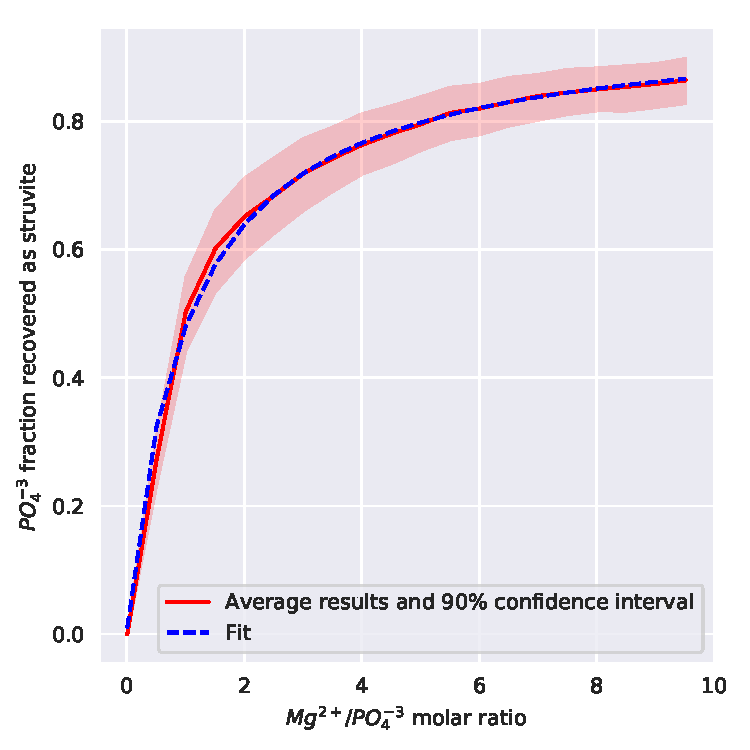
\includegraphics[width=\textwidth]{gfx/AppendixB/plotStrYield_Mg}
		\caption{$x_{struvite \left(PO_{4}^{3-}\right)}$}
		\label{fig:estimation_Mg_value}
	\end{subfigure}
%	\caption{Evolution phosphorus as phosphate fraction recovered as struvite and calcium fraction recovered as precipitates along $\text{Mg}^{2+}/\text{PO}_{4}^{3-}$ molar ratio values considering 50 different composition data sets.}
%\end{figure}
%	%	\quad
%\begin{figure}[h]\ContinuedFloat
%	\centering
	\begin{subfigure}[t]{0.25\textheight}
		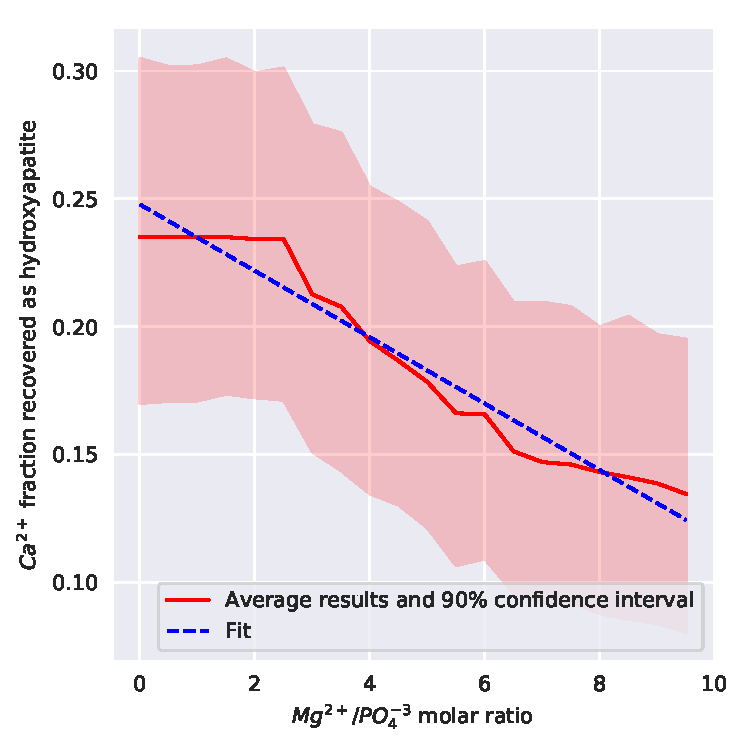
\includegraphics[width=\textwidth]{gfx/AppendixB/x_plotHAPYield_Mg} 
		\caption{Hydroxyapatite}
		\label{fig:Mg_influence_HAP}
	\end{subfigure} 
	%	\quad
	\begin{subfigure}[t]{0.25\textheight}
		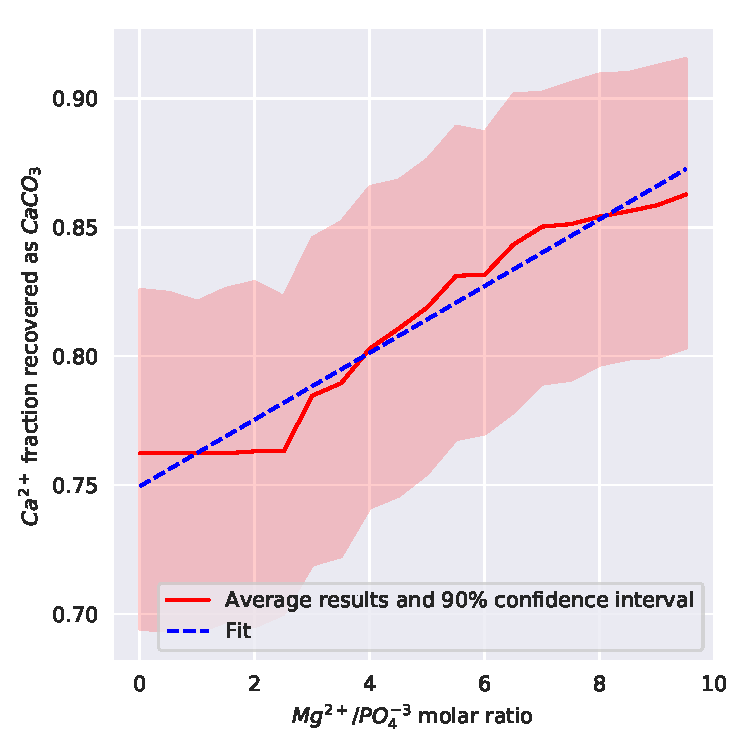
\includegraphics[width=\textwidth]{gfx/AppendixB/x_plotCaCO3Yield_Mg}
		\caption{Calcium carbonate}
		\label{fig:Mg_influence_CaCO3}
	\end{subfigure}
	
	\caption{Evolution phosphorus as phosphate fraction recovered as struvite and calcium fraction recovered as precipitates along $\text{Mg}^{2+}/\text{PO}_{4}^{3-}$ molar ratio values considering 50 different composition data sets.}
	\label{fig:estimation_Mg_ca}
\end{figure}
%\end{sidewaysfigure}

\clearpage
\subsubsection{Influence of calcium}
\begin{figure}[h] 
	\centering
	\begin{subfigure}[t]{0.25\textheight}
		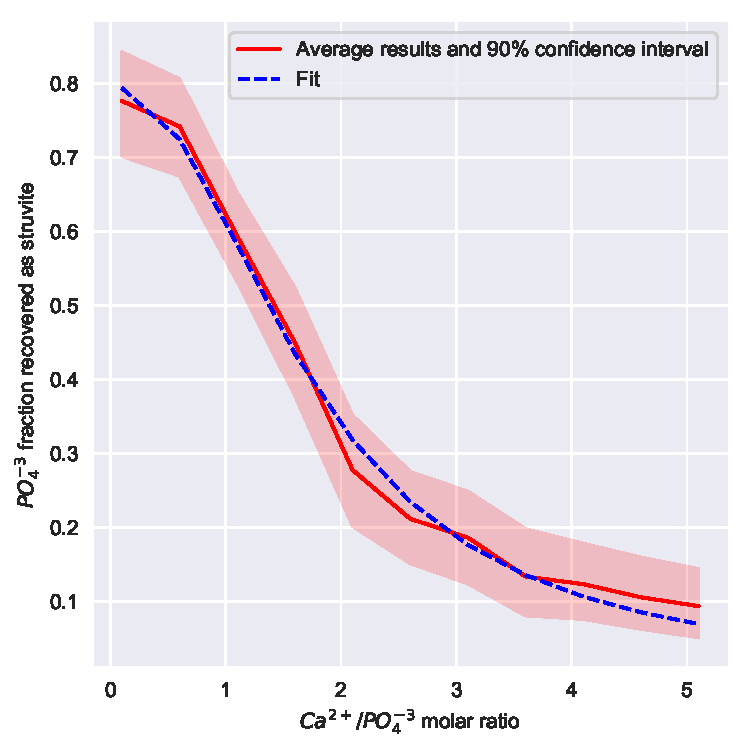
\includegraphics[width=\textwidth]{gfx/AppendixB/plotStrYield_Ca}
		\caption{$x_{struvite \left(PO_{4}^{3-}\right)}$}
		\label{fig:estimation_Ca_value}
	\end{subfigure}
	%	\quad
	\begin{subfigure}[t]{0.25\textheight}
		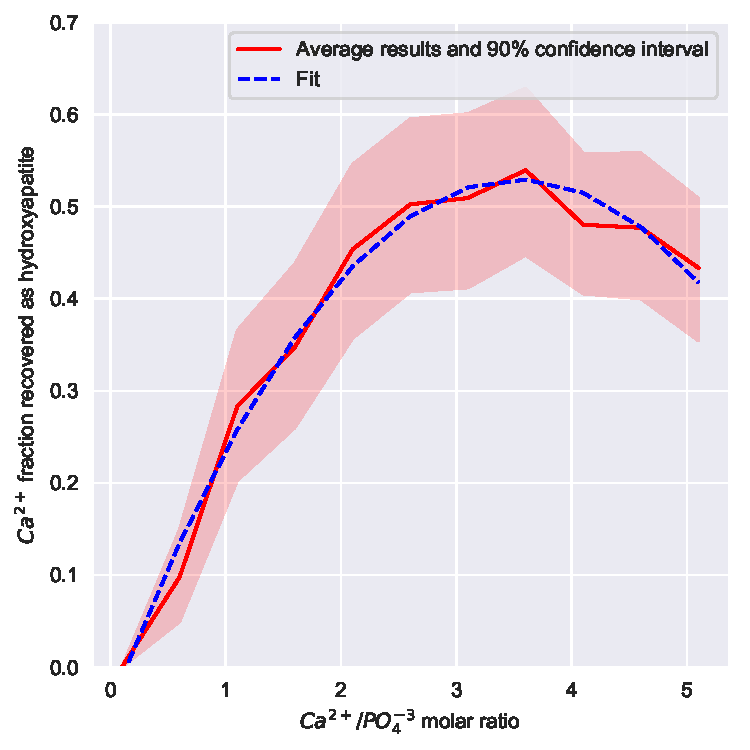
\includegraphics[width=\textwidth]{gfx/AppendixB/x_plotHAPYield_Ca} 
		\caption{Hydroxyapatite}
		\label{fig:estimation_Ca_HAP}
	\end{subfigure} 
	%	\quad
	\begin{subfigure}[t]{0.25\textheight}
		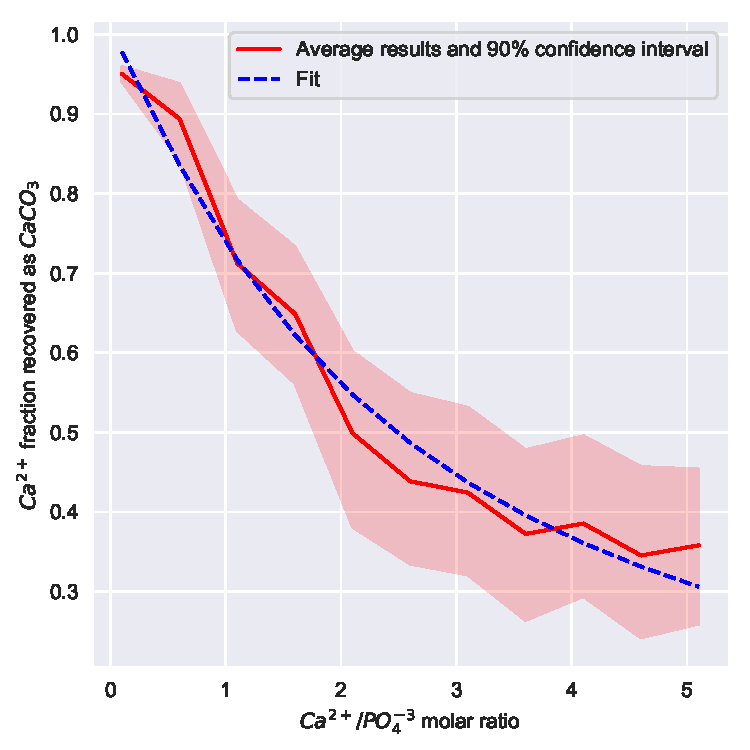
\includegraphics[width=\textwidth]{gfx/AppendixB/x_plotCaCO3Yield_Ca}
		\caption{Calcium carbonate}
		\label{fig:estimation_Ca_CaCO3}
	\end{subfigure}
	
	\caption{Evolution of phosphorus as phosphate fraction recovered as struvite and calcium fraction recovered as precipitates along $\text{Ca}^{2+}/\text{PO}_{4}^{3-}$ molar ratio values considering 50 different composition data sets.}
	\label{fig:estimation_Ca_ca}
\end{figure}

\clearpage
\subsubsection{Influence of alkalinity}
\begin{figure}[h] 
	\centering
	\begin{subfigure}[t]{0.25\textheight}
		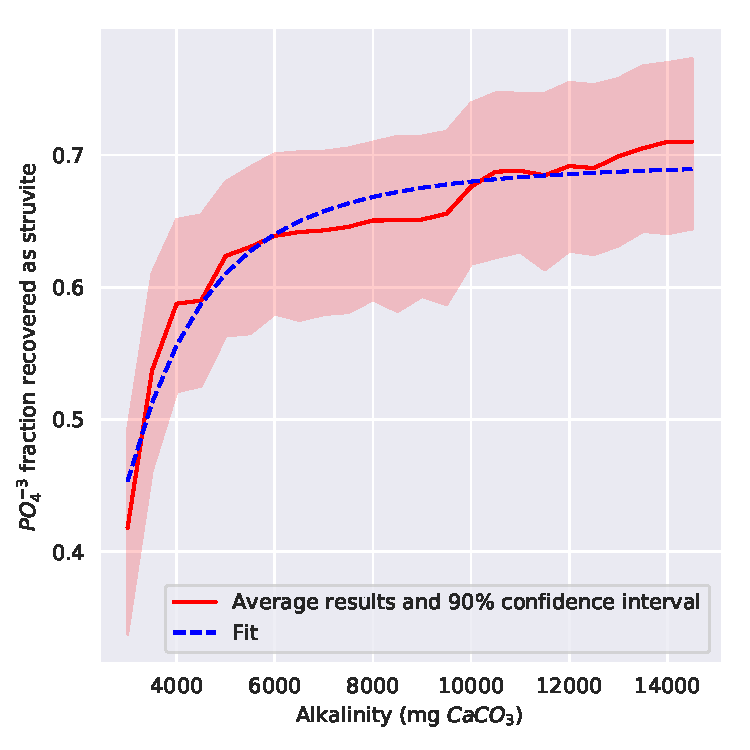
\includegraphics[width=\textwidth]{gfx/AppendixB/plotStrYield_Alk}
		\caption{$x_{struvite \left(PO_{4}^{3-}\right)}$}
		\label{fig:estimation_Alk_struviteYield}
	\end{subfigure}
	%	\quad
	\begin{subfigure}[t]{0.25\textheight}
		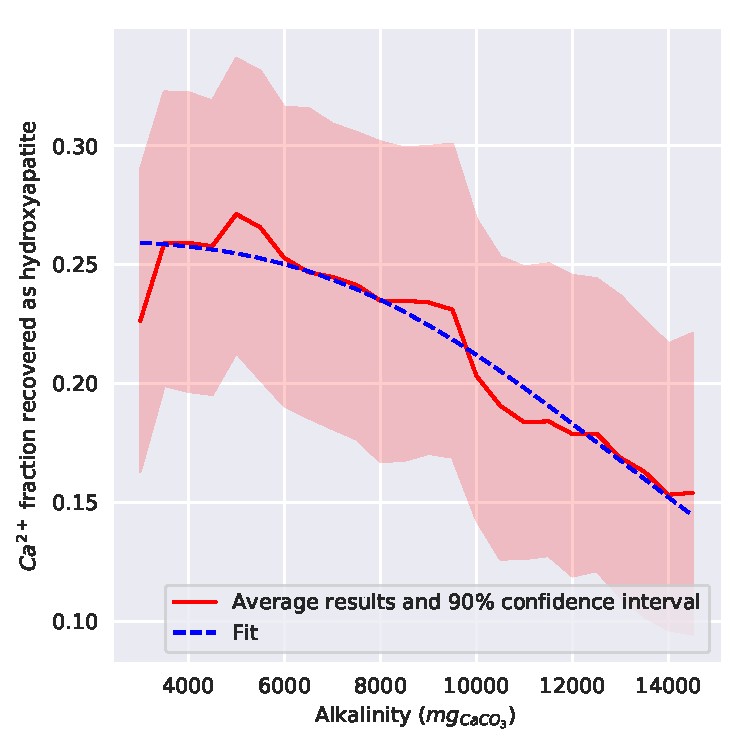
\includegraphics[width=\textwidth]{gfx/AppendixB/x_plotHAPYield_Alk} 
		\caption{Hydroxyapatite}
		\label{fig:estimation_Alk_HAP}
	\end{subfigure} 
	%	\quad
	\begin{subfigure}[t]{0.25\textheight}
		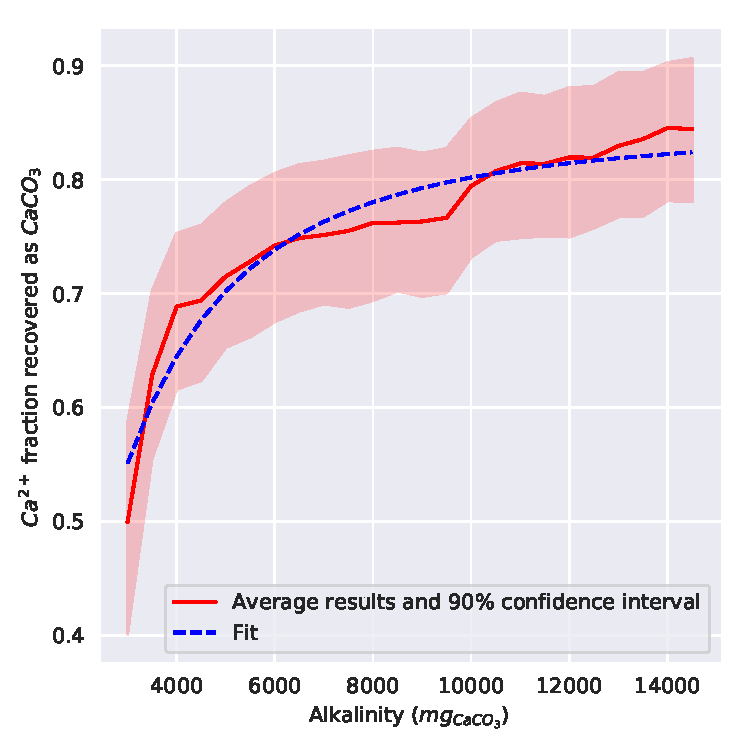
\includegraphics[width=\textwidth]{gfx/AppendixB/x_plotCaCO3Yield_Alk}
		\caption{Calcium carbonate}
		\label{fig:estimation_Alk_CaCO3}
	\end{subfigure}
	
	\caption{Evolution of phosphorus as phosphate fraction recovered as struvite and calcium fraction recovered as precipitates among alkalinity values considering 50 different composition data sets.}
	\label{fig:estimation_Alk}
\end{figure}

\clearpage

\section*{Bibliography}
\addcontentsline{toc}{section}{Bibliography}

\printbibliography[heading=none]
\end{refsection}

%\begin{lstlisting}[float=b,language=Pascal,frame=tb,caption={A floating example (\texttt{listings} manual)},label=lst:useless]
%for i:=maxint downto 0 do
%begin
%{ do nothing }
%end;
%\end{lstlisting}

